\documentclass[a4paper]{article}
\usepackage{graphicx}
\usepackage{color}
\usepackage{enumerate}
\usepackage{multirow}
\raggedbottom
\begin{document}


% this is to display answers
\newcommand{\answer}[1]{
  \textcolor{red}{#1}
}
% comment out line below to show answers
\ifdefined\showanswers
\else
  \renewcommand{\answer}[1]{}
\fi
\title{Numeracy Evaluation \answer{with answers}}
\author{Organic Trader Pty Ltd}

\maketitle
\noindent This evaluation is designed to give us an indication of your maths abilities. Please answer the following questions as best you can. If you don't understand something please ask.

\hspace{5mm}

\noindent Name: \rule{3cm}{0.2pt}

\hspace{5mm}

\noindent Date: \rule{3cm}{0.2pt}



\section{No calculator to be used}

Please answer the following questions without the use of a calculator. You may use the space provided for doing your calculations.

\begin{enumerate}
\item \begin{math}  32 + 12 = \end{math} \answer{44}
\item \begin{math}  12 \times 8 = \end{math} \answer{96}
\item   20\%  of 40 = \answer{8}
\item \begin{math}  72 - 18 = \end{math} \answer{54}
\item \begin{math}  32 \times 1.5 = \end{math} \answer{48}
\item \begin{math}  \frac{1}{2} + \frac{1}{4} = \end{math}
  \answer{$\frac{3}{4}$ or 0.75}
\item \begin{math}  \frac{1}{2} \times \frac{1}{4} = \end{math}
  \answer{$\frac{1}{8}$ or 0.125}
\item Round the following numbers to two decimal places: 
  \begin{enumerate}\addtolength{\itemsep}{1\baselineskip}
    \item 12.3424 \answer{12.34}
    \item 42.6395 \answer{42.64}
    \item 633.77872 \answer{633.78}
    \item 0.5666256 \answer{0.57}
    \item 2.999 \answer{3.00}
    \item 5013.3333 \answer{5013.33}
    \item 3.114999 \answer{3.11}
    \item 17.10059 \answer{17.10}
  \end{enumerate} 
\item In Microsoft Excel, it is useful to be able to sum the numbers in a column. In cell A7, please write the forumla to calculate the sum of all the numbers listed.

\makebox[\textwidth][c]{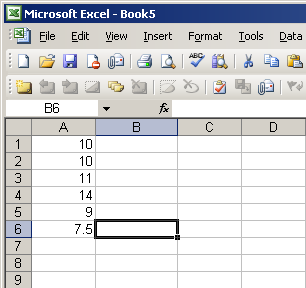
\includegraphics[width=1\textwidth]{excel-screenshot}}

\newpage
\item It is also sometimes useful to have a running total for a list of numbers. Please write the formulas in column B to calculate the running totals for the numbers listed.

\makebox[\textwidth][c]{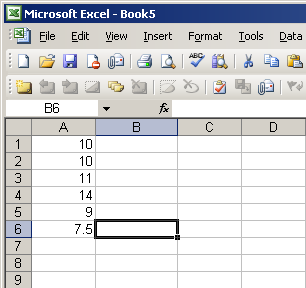
\includegraphics[width=1\textwidth]{excel-screenshot}}

\end{enumerate}
\newpage
\section{Calculator to be used}
Please answer the following questions. You may use a calculator to help you answer the questions in this section.
\begin{enumerate}\addtolength{\itemsep}{1\baselineskip}

\item \begin{math} 27284 + 36723 = \end{math} \answer{64007}
\item \begin{math} 17.71 \times 12.45 = \end{math} \answer{220.4895}
\item \begin{math} 272 - 89 = \end{math} \answer{183}
\item \begin{math} 1027 \div 13 = \end{math} \answer{79}
\item \begin{math} 137 + 55 \times 12 = \end{math} \answer{797} 
\item One of our products, Cocolo Dark Orange Chocolate comes in boxes of 25 bars called inners. Those inners are then packed into larger cartons called outers. There are 10 inners to the outer. 

A customer orders 275 bars of chocolate. How many inners and outers will we ship to them? 
\answer{1 outer plus 1 inner}


\item Another product comes as 12 units per carton. 

A customer orders 36 units. How many cartons should we ship to them?

 \answer{3 cartons}

\item In Australia, GST is set at 10\%. If a product is priced at \$19.22 excluding GST, what is the price including GST?

\answer{\$21.142}

\item When processing orders it is vital that the details of the
  order are entered correctly. Please compare the order code and order quantities in columns A
  and B and highlight any errors you may find.

\begin{table}
\begin{tabular}{lr|lrl}
\multicolumn{2}{c}{Column A} & \multicolumn{2}{c}{Column B}\\ \hline
Product Code &Qty&Product Code&Qty&\answer{Error}\\
\hline
6002010&1&6020010&1&\answer{Error in Product Code}\\
6003351&1&6003351&1&\answer{  }\\
6003401&1&6003401&1&\answer{  }\\
6003402&1&6003402&1&\answer{  }\\
6003405&2&6003405&2&\answer{  }\\
6004302&1&6004302&1&\answer{  }\\
6004341&1&6004314&1&\answer{  Error in Product Code}\\
6004361&1&6004361&1&\answer{ }\\
6004303&3&6004303&8&\answer{  Error in Qty}\\
6005422&1&6005422&1&\answer{ }\\
6008001&1&6008001&1&\answer{ }\\
6008005&1&6008005&1&\answer{ }\\
6008011&1&6008011&1&\answer{ }\\
6220002&1&6220002&1&\answer{ }\\
6302002&1&6302002&1&\answer{ }\\
6302005&1&6302005&1&\answer{ }\\
6303002&1&6303002&1&\answer{ }\\
6351306&1&6351306&1&\answer{ }\\
6591201&1&65912201&1&\answer{  Error in Product Code}\\
6591207&1&6591207&1&\answer{ }\\
6601006&1&6601006&1&\answer{ }\\
6901013&1&6901013&1&\answer{ }\\
6901014&1&6901014&1&\answer{ }\\
6901017&1&6901017&1&\answer{ }\\
6901021&2&6901021&2&\answer{ }\\
6901022&2&6901002&2&\answer{  Error in Product Code}\\
6901031&1&6901031&1&\answer{ }\\
6901032&1&6901032&1&\answer{ }\\
6901041&6&6901041&6&\answer{ }\\
6901042&5&6901042&5&\answer{ }\\
6901055&2&6901555&2&\answer{  Error in Product Code}\\
6901061&2&6901061&2&\answer{ }\\
6901063&1&6901063&1&\answer{ }\\
6901071&2&6901071&2&\answer{ }\\
6901079&1&6901079&1&\answer{ }\\
6902232&1&6902232&1&\answer{ }\\
6902233&1&6902233&1&\answer{ }\\
6902241&1&6902241&1&\answer{ }\\
6902242&1&6902242&1&\answer{ }\\
6902752&1&6902752&1&\answer{ }\\
6904007&1&6904007&1&\answer{ }\\
6911021&1&6911021&1&\answer{ }\\
6921001&1&6921001&1&\answer{ }\\
8451033&7&8451033&1&\answer{  Error in Product Qty}\\
8451034&7&8451034&7&\answer{ }\\
8451035&7&8451035&7&\answer{ }\\
8451036&6&8451836&6&\answer{  Error in Product Code}\\
8451205&4&8451205&4&\answer{ }\\
\end{tabular}
\end{table}


\end{enumerate}
\end{document}

%%% Local Variables:
%%% mode: latex
%%% TeX-master: t
%%% End:
